 \chapter{Numerical Experiments}
\section{Comparison of mesh lifting operators}
Mesh lifting operators are essential for numerical stability of fluid-structure interaction. If the fluid mesh doesn't conform with the solid deformation, mesh entanglement increases with the possibility of numerical instabilities. In general, mesh models have shown to be either robust concerning mesh entanglements at the cost of computational time, or computational efficient with less robustness \cite{MM2016}. However, computational efficiency has proven not only to be dependent of the complexity of model, but also the regularity of the fluid mesh, reducing Newton iterations needed per time step \cite{Wickb}. In this section I compare the mesh moving models from section 3.1.4. for the FSI-3 benchmark. The linear elastic model was found not applicable in section 4.2.3. Therefore, only the Laplace and biharmonic lifting operators will be considered, comparing vertical displacement of the elastic flag, regularity of the fluid mesh, and number of Newton iterations per time step. To evaluate the regularity of the fluid mesh, the minimum value of the Jacobian of the deformation gradient have been considered in \cite{Wickb}. The Jacobian serves as a measure of mesh entanglement, meaning if $J_f \geq 0$, there are no crossing cells in the fluid mesh. 
\begin{align*}
{J}_f = det(\bat{F}_f) =  det(I + \hat{\nabla} \bat{u}_f)
\end{align*}
where $I$ is the identity matrix and $ \bat{u}_f$ is the fluid mesh deformation.  
\newpage

\subsection*{Results}
Figure \ref{fig:minjcomp} shows a comparison the mesh moving models at the time interval  $t = [0, 5]$, when a stable periodic solution is obtained. As shown in the middle figure all models shows a minima of mesh regularity at $3.8s < t < 4.2$, which is expected due to the largest deformation of the elastic flag. A larger number of Newton iterations for all models shows are needed at each time step, when the elastic flag starts oscillating for $t > 3s$. The biharmonic lifting operator is superior in terms of number of iterations need per time step, and mesh regularity in comparison with the Laplace model. Further, the biharmonic 2 model shows better mesh regularity than biharmonic 1, but shows equal behavior in terms of Newton iterations. Recall, the biharmonic 2 operator allows tangential mesh motion at the boundaries, while the biharmonic 1 model constraining mesh motion in both perpendicular and tangential direction. For all models, no distinct difference in deformation of the y-component is found.

\begin{figure}[h!]
        \centering
    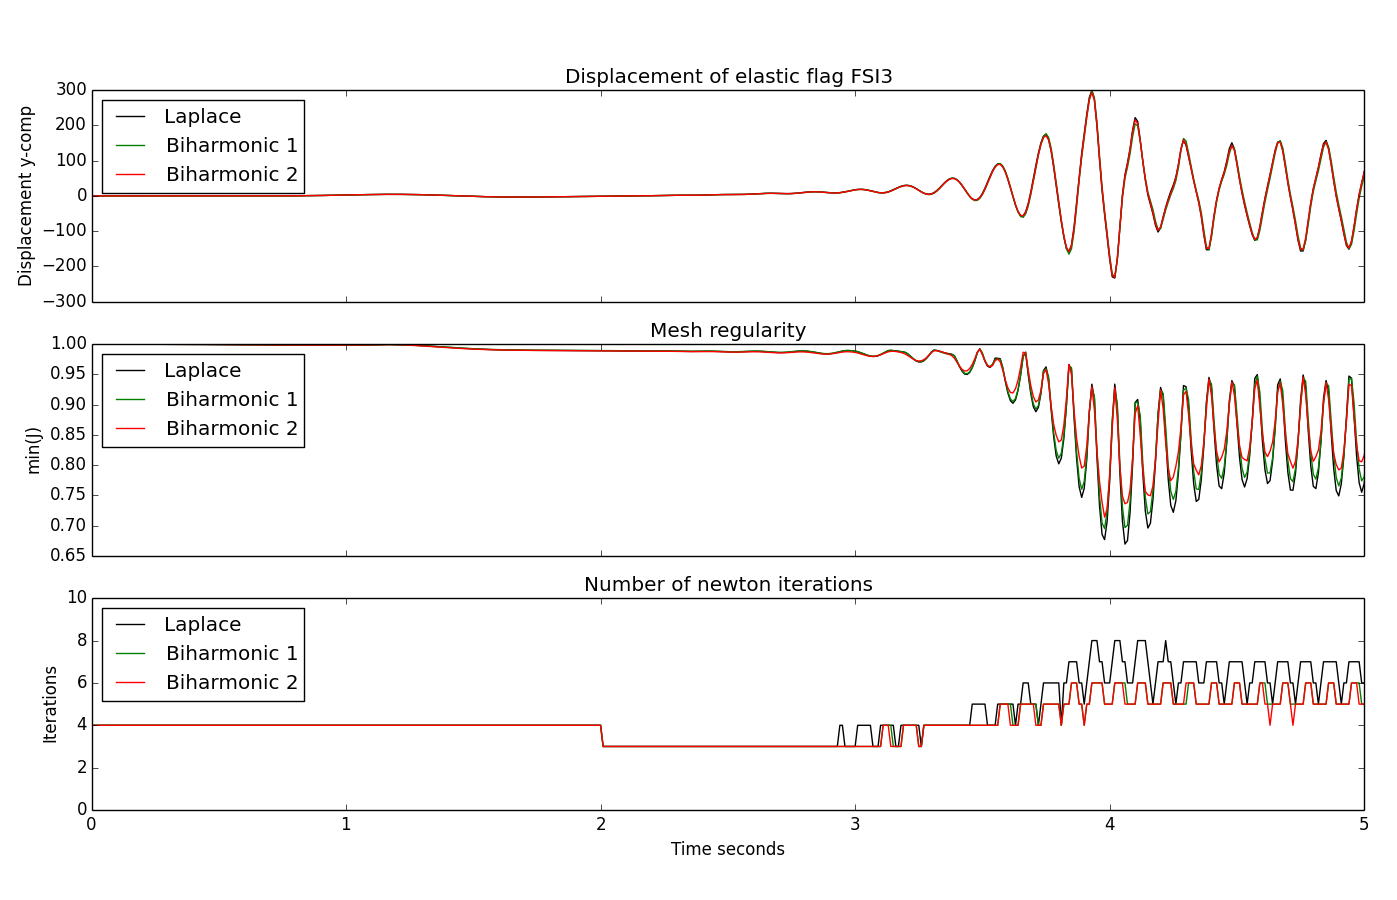
\includegraphics[scale=0.4]{./Fig/minjcompare.png} \\
      \caption{Investigation of mesh moving models for the FSI3 benchmark in the time interval $t \in [0, 5]$, comparing vertical displacement of elastic flag, mesh regularity, and number of Newton iterations.}
      \label{fig:minjcomp}
\end{figure}

\subsection*{Discussion}
The numerical results confirms biharmonic models produce a better regularity of the fluid mesh cells, which in turn reduces the number of Newton iterations needed per time step. However,  better evolution of mesh cells is by no means necessary for solving the FSI-3 problem. Therefore, the Laplace model remains a good choice, and its simplicity is preferable in terms of computational time (a topic to be discussed in section ~\ref{fig:cncomp1} 
~\ref{sec:opti} ).
\newpage
\section{Investigation of long term temporal stability}
One of the main challenges for constructing time-stepping schemes for ALE-methods, is the additional non-linearity introduced by the domain-velocity term in the fluid problem \cite{Formaggia2004}:
\begin{align}
\ha{J}_f (\hat{F}_f^{-1}(\bat{v}_f - \pder{\ha{T}_f}{t}) \cdot \hat{\nabla}) \bat{v}_f
\end{align} 
Closer inspection of the convective term reveal spatial and temporal differential operators depending non-linearly on one another. These differential operators often appear separated, making discretization of a general time-stepping scheme not directly intuitive. The domain velocity $ \pder{\ha{T}_f}{t}$ have proven to effect the stability of first and second-order accurate time stepping schemes on fixed domains, but to what extent remains unclear  \cite{Formaggia2004, Formaggia1991}. The second order Crank-Nicolson used in this thesis, have also shown to suffer from temporal stability for long-term simulations of fluid problems. The unconditionally stable Crank-Nicolson scheme is restricted by the condition \cite{Wick2013a}:
\begin{align}
k \leq ch^{\frac{2}{3}} 
\end{align}
Were c is a constant, while k and h are the time-step and a mesh-size parameters. While for the stability of the time derivative of the ALE-mapping, no accurate restriction is obtained (althought thouroughly explored in \cite{Formaggia2004}). As a result, time step restriction is necessary to ensure that numerical stability  \cite{Formaggia2004}. The temporal stability for the implicit Crank-Nicolson scheme, for the validation benchmark chosen in this thesis, was studied in  \cite{Richter2015}. The criteria for the numerical experiments was to obtain a stable solution in the time interval of 10 seconds, by temporal and spatial refinement studies. Following the ideas outlined in \cite{Richter2015}, a second order scheme based on the Crank-Nicolson yields two possibilities:
\begin{discr}
\textit{Crank?Nicolson secant method }
\begin{align*}
\Big[\frac{\ha{J}(\bat{u}^{n}) \bat{\nabla} \bat{v}^{n} \bat{F}_W^{-1}}{2} 
+ \frac{\ha{J}(\bat{u}^{n-1}) \bat{\nabla} \bat{}v^{n-1} \bat{F}_W^{-1}}{2} \Big] 
\frac{\bat{u}^{n} - \bat{u}^{n-1}}{k}
\end{align*} 
\label{eq:cn1}
\end{discr}
\begin{discr}
\textit{Crank?Nicolson midpoint-tangent method}
\begin{align*}
\Big[\frac{\ha{J}(\bat{u}_{cn}) \bat{\nabla} \bat{v}_{cn} \bat{F}_W^{-1}}{2} \Big] 
\frac{\bat{u}^{n} - \bat{u}^{n-1}}{k} \hspace{4mm}
\bat{u}_{cn} = \frac{\bat{u}^{n} + \bat{u}^{n-1}}{2} \hspace{2mm}
\bat{v}_{cn} = \frac{\bat{v}^{n} + \bat{v}^{n-1}}{2}
\end{align*} 
\label{eq:cn2}
\end{discr}
\newpage
The numerical experiments showed very similar performance for Discretization  ~\ref{eq:cn1}, ~\ref{eq:cn2}, and significant differences of long-term temporal stability was not found. However, spatial and temporal refinement showed the implicit Crank-Nicolson suffered from long-term stability problems for certain time steps. Choosing the time step $k = [0.005, 0.003]$, the FSI-3 problem (Section  ~\ref{sec:fsi3} ) suffered from numerical instabilities. Interestingly, the instabilities occurred earlier in simulation time for increasing mesh refinement. A similar experiment in  \cite{Wicka}, showed reducing the time step $k = 0.001$  yield stable long-time simulation for both  Discretization  ~\ref{eq:cn1} and ~\ref{eq:cn2}. \\
To overcomes the numerical instabilities two approaches have been suggested in the literature,  the \textit{shifted Crank-Nicolson}  and the \textit{fracstep method}  \cite{Richter2015, Wicka, Wick2013a}.  In this thesis the shifted Crank-Nicolson scheme was considered, introducing stability to the overall system by shifting the centered scheme  by $\theta = \frac{1}{2} + k$. If the shift is dependent of the time-step \textit{k} such that $\frac{1}{2} \leq \theta \leq \frac{1}{2} + k$, the scheme will be of second order \cite{Richter2015}. \\
\subsection{Results}
A numerical investigation of long term numerical stability is shown in Figure ~\ref{fig:cncomp1}, ~\ref{fig:cncomp2}, where the shifted Crank-Nicolson scheme $\theta = \frac{1}{2} + \Delta t$, is compared the original Crank-Nicolson $\theta = \frac{1}{2}$. The shifted surpasses the original Crank-Nicolson scheme in terms of temporal stability, for all time steps. In Figure ~\ref{fig:cncomp2}, the shifted Crank-Nicholson scheme retain long-time temporal stability for  $\Delta t = 0.01$.. While for the ordinary Crank-Nicholson scheme, numerical experiments showed choosing $\Delta t = 0.001$ was necessarily to ensure stability, confirming the results found in \cite{Wicka}.  \\
Figure ~\ref{fig:cncomp1} shows choosing $\Delta t \in [0.2, 0.1]$ results in a steady-state solution, which can be explained by influence the solid problem. A centered Crank-Nicolson scheme $\theta= \frac{1}{2}$ is energy preserving, meaning no energy is dissipated from the system. Since the shifted Crank-Nicolson scheme is not centered, the amount of dissipated of energy is related to the time step. If the time step is sufficiently high such as $\Delta t \in [0.2, 0.1]$, the scheme will dissipate energy at a higher rate. Therefore, no periodic oscillation of the elastic flag is obtained. The validation of the solid solver shows the difference of energy dissipation for a centered and backward numerical scheme. Given the same solid parameters, a steady-state solution is obtained for CSM-1 ($\theta = 1.0 $), while CSM-3 yields a periodic solution CSM-3 ($\theta = \frac{1}{2}$ ), shown in Figure ~\ref{fig:csm1scm3} .\\
For $\Delta t \in [0.05, 0.02]$, the shifted Crank-Nicolson scheme is close to centered, meaning energy is nearly preserved in the structure. However, the Newton-solver diverges before full time interval of 10 seconds is finished. Surprisingly, a finer time step $\Delta t = 0.02$ fails at an earlier stage than $\Delta t = 0.05$. The breakdown is not due to mesh entanglement of the ALE-mapping, but divergence of Newton method itself\cite{Richter2015}. It is believed the divergence of the Newton solver is linked to the influence of the domain velocity, by the research found in \cite{Formaggia2004}, but no clear time step restriction is obvious. Hence, several publications indicates choosing time step for a shifted Crank-Nicolson scheme is based on trial and error \cite{Wicka, Wick2013a}. 
\begin{figure}[h!]
        \centering
    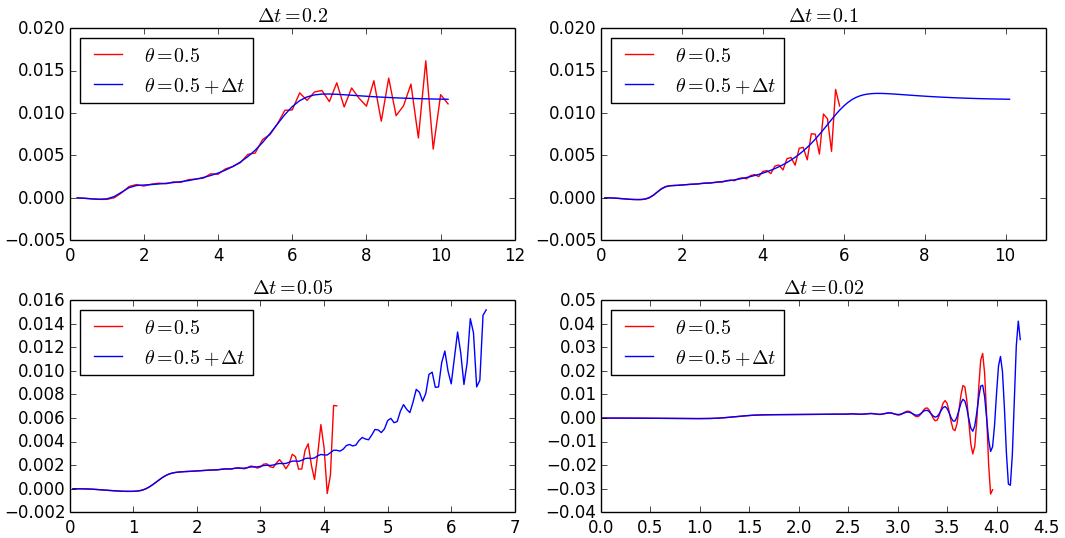
\includegraphics[scale=0.6]{./Fig/thetacheck.png} \\
      \caption{Investigation of long term numerical stability for the FSI3 benchmark in the time interval $t \in [0, 10]$, comparing the shifted and centered Crank-Nicolson scheme. }
\label{fig:cncomp1}
\end{figure}
\begin{figure}[h!]
        \centering
    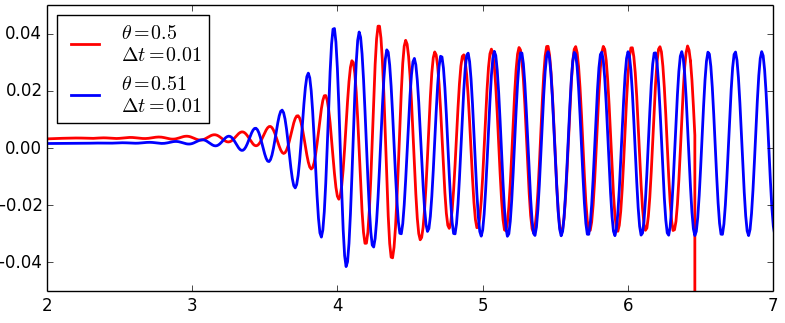
\includegraphics[scale=0.6]{./Fig/besttheta.png}
      \caption{Investigation of long term numerical stability for the FSI3 benchmark in the time interval $t \in [0, 10]$,  comparing the shifted and centered Crank-Nicolson scheme. }
\label{fig:cncomp2}
\end{figure}
\newpage
\begin{figure}[h!]
        \centering
    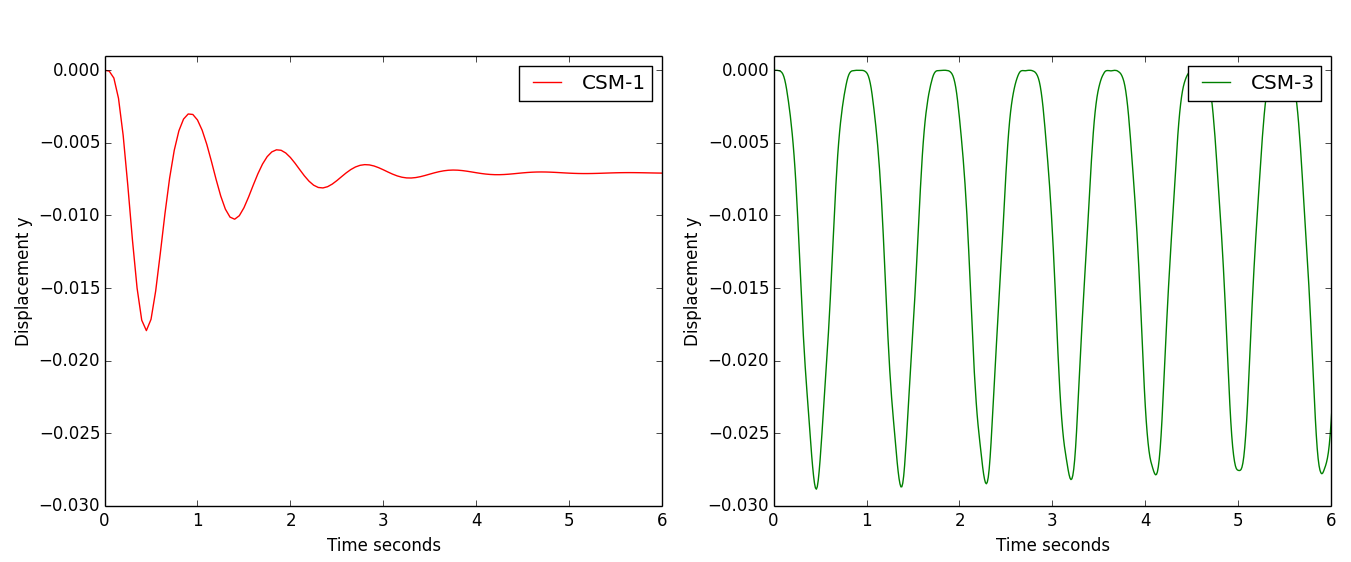
\includegraphics[scale=0.4]{./Fig/thetacompare.png}
      \caption{A comparison of a centered Crank-Nicolson scheme and backward Euler scheme, using the structure validation benchmark for the time interval  $t \in [0, 6]$. Using the same structure parameters, a backward-Euler scheme $\theta = 1$ yields steady-state solution for CSM-1, while a periodic solution is observed for CSM-3 using a centered scheme $\theta = \frac{1}{2}$  }
\label{fig:csm1scm3}
\end{figure}
\newpage
\section{Optimization of the Newton solver}
\label{sec:opti}
\textit{Software profiling} is a dynamic program analysis, with the purpose of finding software sections which can be optimized. In scientific computing, software profiling often focuses on minimizing memory usage or executing speed, by collecting performance data to identify bottlenecks. A \textit{bottleneck} is a term used when the total performance of a complete implementation is limited to small code fragments, accounting for the primary consumption of computer resources. For many applications, one can often assume the usage of resources follows the \textit{The Pareto principle}. Meaning that for different types of events, roughly 80\% of the effects come from 20\% of the causes. An analogy to computational sciences it that 80\% of the computational demanding operations comes from 20\% of the code. In this thesis, software profiling identified the bottleneck to be the Newton solver, using roughly $\sim 98 \%$ of the total computational time for each individual numerical experiment. For a full simulation of the FSI-3 problem considered in Chapter ~\ref{sec:fsi3}, on a courses mesh with time step $k = 0.01$, the total computation time was initially 68 hours. With additional spatial and temporal refinement study of four mesh moving models, it became clear that the whole process would be too time consuming. Optimization of the Newton solver was therefore eminent to complete the initial goals set for this thesis. \\
Newtons method can be written as,
\begin{align}
\nabla \mathbf{F}(\mathbf{x}_n)(\mathbf{x}_n - \mathbf{x}_0) = - \mathbf{F}(\mathbf{x}_n)
\label{eq:newton}
\end{align}
where $\mathbf{F}$ is the residue of the variational formulation, $\mathbf{x}_n$, $\mathbf{x}_0$ is vector, and $ \nabla \mathbf{F}$ is the Jacobian of the residue. The Newton method can be divided into two main computational demanding operations.
\begin{itemize}
\item \textbf{Jacobian assembly} \\
The construction of the Jacobian matrix $\nabla \mathbf{F}(\mathbf{x}_n)$ of the total residue $\mathbf{F}(\mathbf{x}_n)$
\item \textbf{Direct solver} \\ 
LU factorization and solving the linear system $\mathbf{Ax} = \mathbf{b}$, where $\mathbf{A} = \nabla \mathbf{F}(\mathbf{x}_n)$ and $\mathbf{b} = - \mathbf{F}(\mathbf{x}_n) $
\end{itemize}
%The \textit{direct solver} proved to be the most demanding operation, using up to $90 \%$ of the computational time at each time step.
The speed-ups methods explored in this thesis are divided into \textit{consistent} and \textit{inconsistent} methods. 
Consistent methods speeds-up the solution process by efficient assembly methods of the linear system ~\ref{eq:newton}. Inconsistent method involves simplifications of the linear system ~\ref{eq:newton}, often at the cost of poor convergence of Newtons method. As a consequence, additional Newton iterations are often necessary for convergence at each time step. 
\newpage
\subsection{Consistent methods}
\subsubsection{Jacobi buffering}
The residue of the FSI problem consists of both linear and non-linear terms, $\mathbf{F} = \mathbf{F}_{lin} + \mathbf{F}_{nonlin}$. For each time step the linear part $\mathbf{F}_{lin}$ remains constant, which only need to be assembled on the first Newton iteration.  The linear parts are then buffered, meaning saved in a separate matrix and added with the assembled non-linear $\mathbf{F}_{nonlin}$ matrix for each Newton iteration at each time step. 
\subsection{Inconsistent methods}    
\subsubsection{Reuse of Jacobian}
Reusing the Jacobian of the residue $\nabla \mathbf{F}(\mathbf{x}_n)$ have two beneficial consequences. First, the 
Jacobian of the residue $\nabla \mathbf{F}(\mathbf{x}_n)$ is only assembled once at each time step. Second, the
LU factorization of the linear system ~\ref{eq:newton} is only needed at the first iteration, as the Jacobian remains constant through the whole time step. The first Newton iteration is therefore solved without simplifications, while the remaining iterations uses an inexact Jacobian which reduces the convergence of the method.
\subsubsection{Quadrature reduce}
The assemble time of the Jacobian greatly depends on the degree of polynomials used in the discretization of the total residual.  The use of lower order polynomials reduces assemble time of the Jacobian at each Newton iteration due decreased size of the Jacobian matrix. The decreased size of the matrix also reduces the time needed for LU-factorization of the linear system ~\ref{eq:newton}. However, the quadrature reduce method leads to an inexact Jacobian which may results to additional iterations. 
\subsubsection{Combining quadrature reduce and Jacobian reuse}
By using the previous inconsistent methods together, the first assembly of the Jacobian is done with lower order polynomials. This combination reduces assembly time of the Jacobian matrix at first iteration, and further speeds up  LU-factorization of the linear system ~\ref{eq:newton}. 
\subsection{Comparison of speedup methods}
% All methods show an increasing number of iterations for $t > 3$,  with a maximum value  at $ 3.8 < t <4.2$.
In Figure ~\ref{fig:lap_it}, all speed-up techniques are compared on the time interval $t = [0, 5]$, for the Laplacian model. Numerical simulations shows how all inconsistent methods increase the number of iterations needed for convergence at each time step, contrary to a consistent naive method. However, the inconsistent methods clearly dominate the time used for a full Newton iteration at each time step, in comparison with the naive approach. The fastest method proved to be the combined method, using $1.5$ hours for solving the full time interval. The naive approach used $17.1$ hours, meaning the combined method resulted in a $91 \%$ speedup. \\
The biharmonic mesh model results in Figure ~\ref{fig:bi_it}, shows  similar observation compared to the Laplacian model. However, the benefit of a better evolution of mesh cells is reflected in the reduced number of iterations needed at each times step, for all methods. The quadrature reduce method even compares to the naive method in terms of iterations. The naive approach computed the whole time interval in $33.87$ hours, while the combined method  $3.46$ hours, a speedup of $89\%$.
\begin{figure}[h!]
 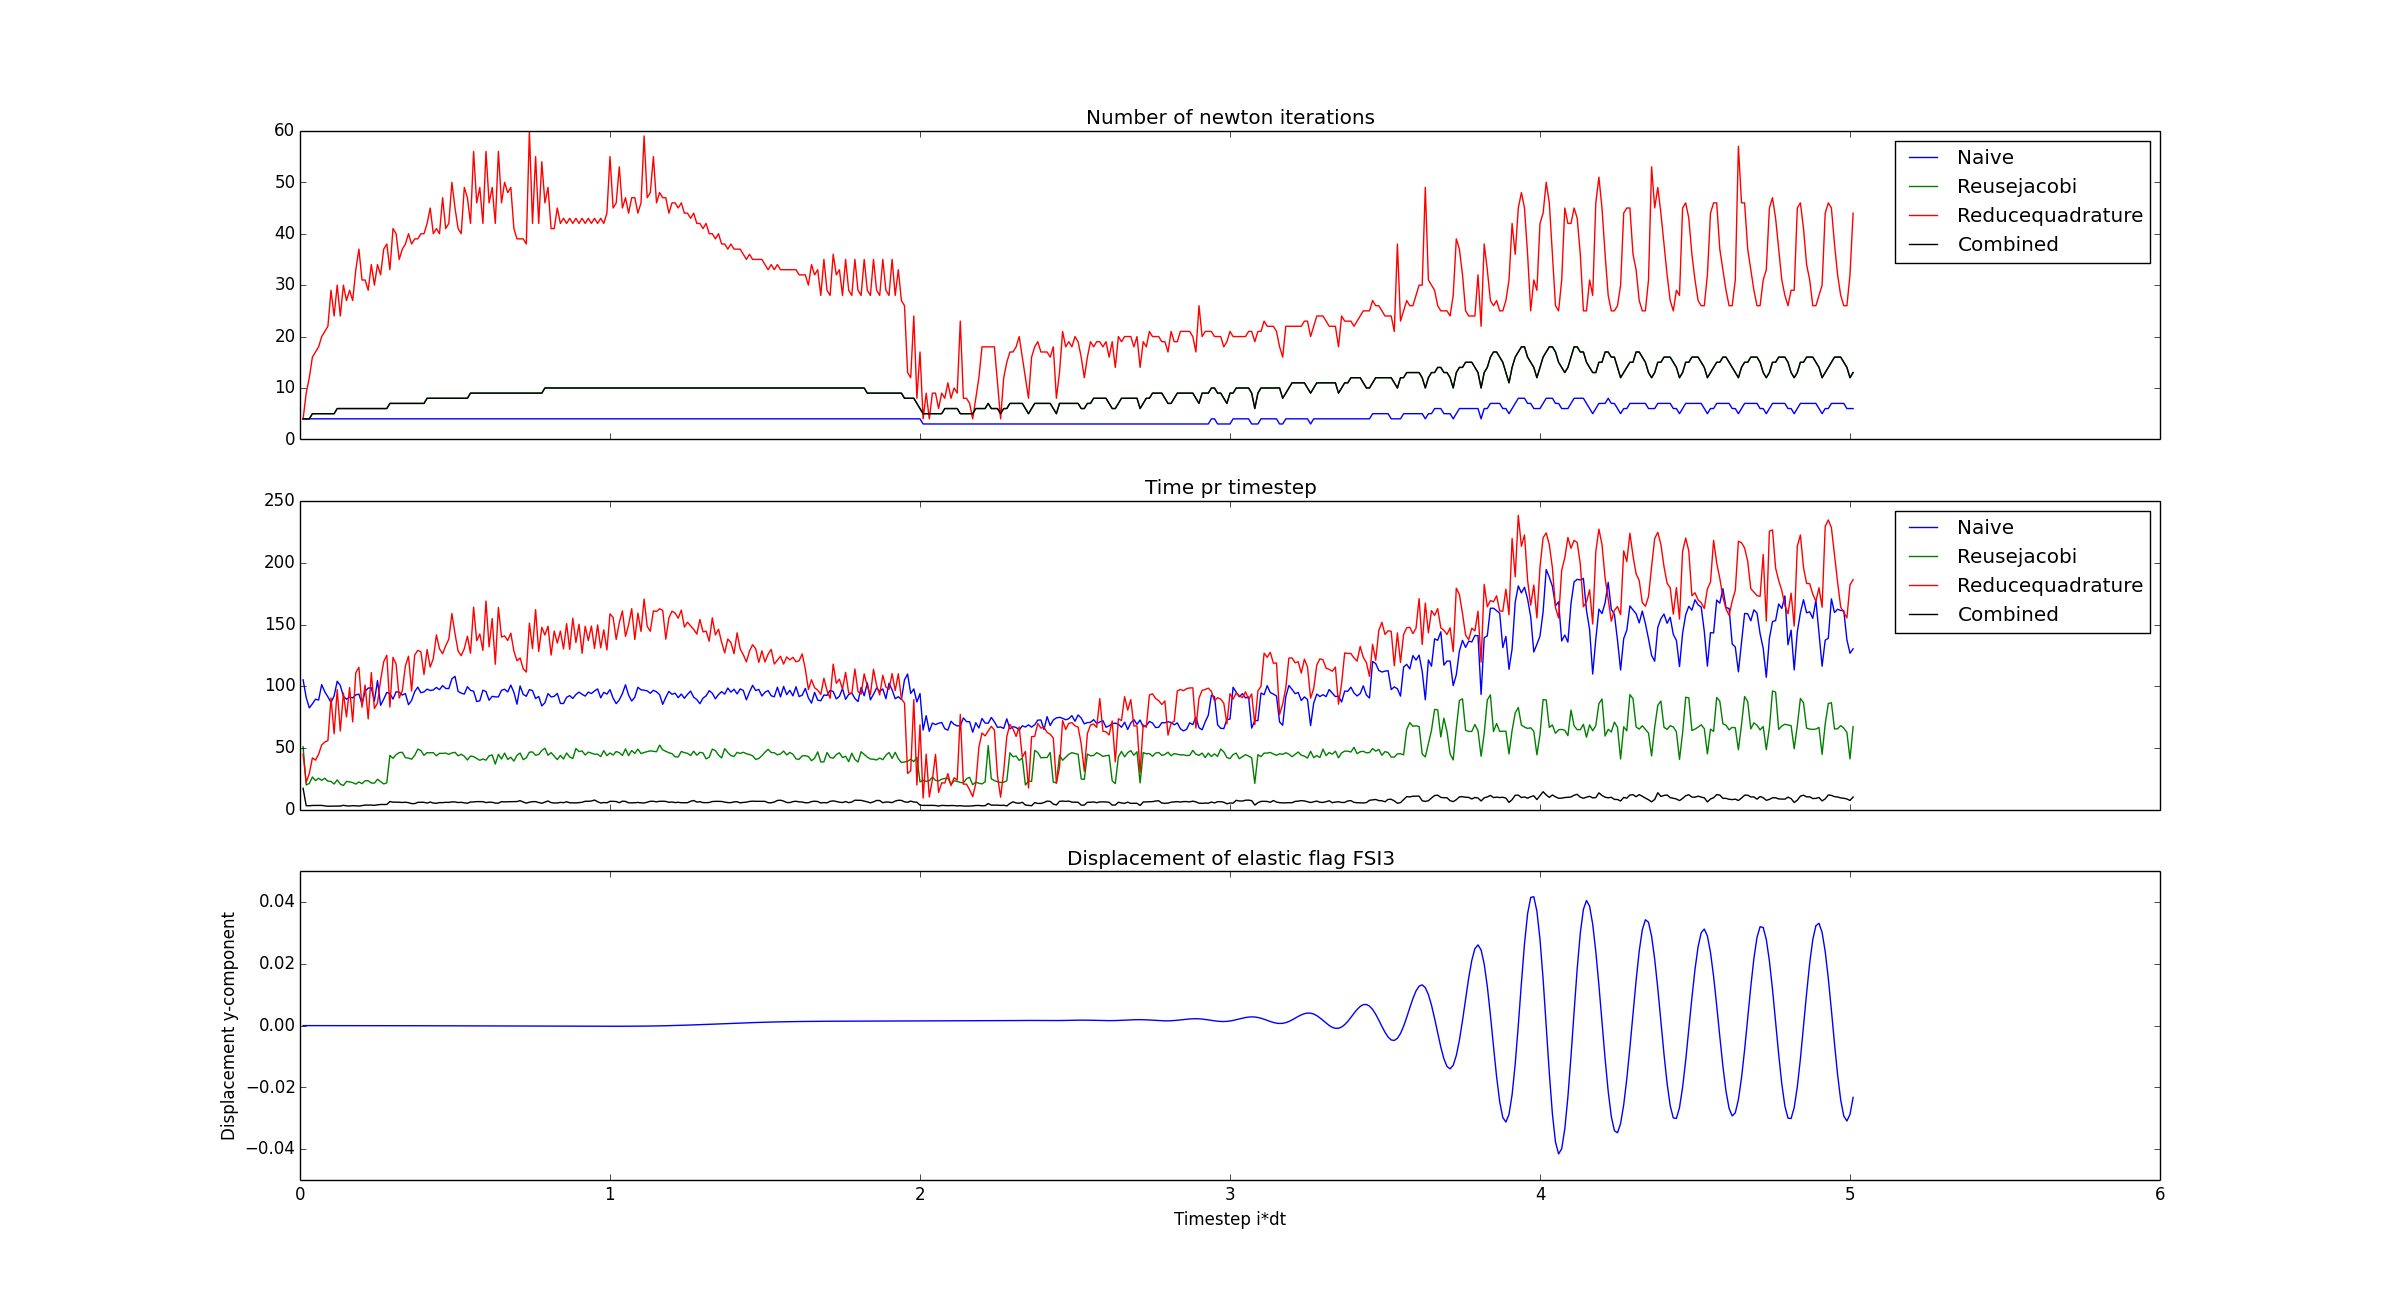
\includegraphics[scale=0.38]{./Fig/itercompare.png}
 \begin{tabular}{ |p{2.8cm}|p{2.2cm}|p{2.4cm}|p{2.4cm}|p{2.4cm}|p{2.4cm}| }
 \hline
  \multicolumn{6}{|c|}{Laplace} \\
 \hline
Implementation & Naive&Buffering&Reusejacobi&Reducequadrature&Combined \\
\hline
 Mean time pr timestep &123.10  & 159.85  & 61.31  & 31.43  & 11.11  \\
\hline
Mean iteration &4.50  & 7.79  & 10.22  & 10.08  & 10.22  \\
\hline
Speedup ratio& -  & 0.12  & 0.50  & 0.74  & 0.91  \\
  \hline
\end{tabular}
 \caption{Comparison of speed-up techniques for the Laplace mesh model.}
 \label{fig:lap_it}
\end{figure}
\newpage
\begin{figure}[h!]
 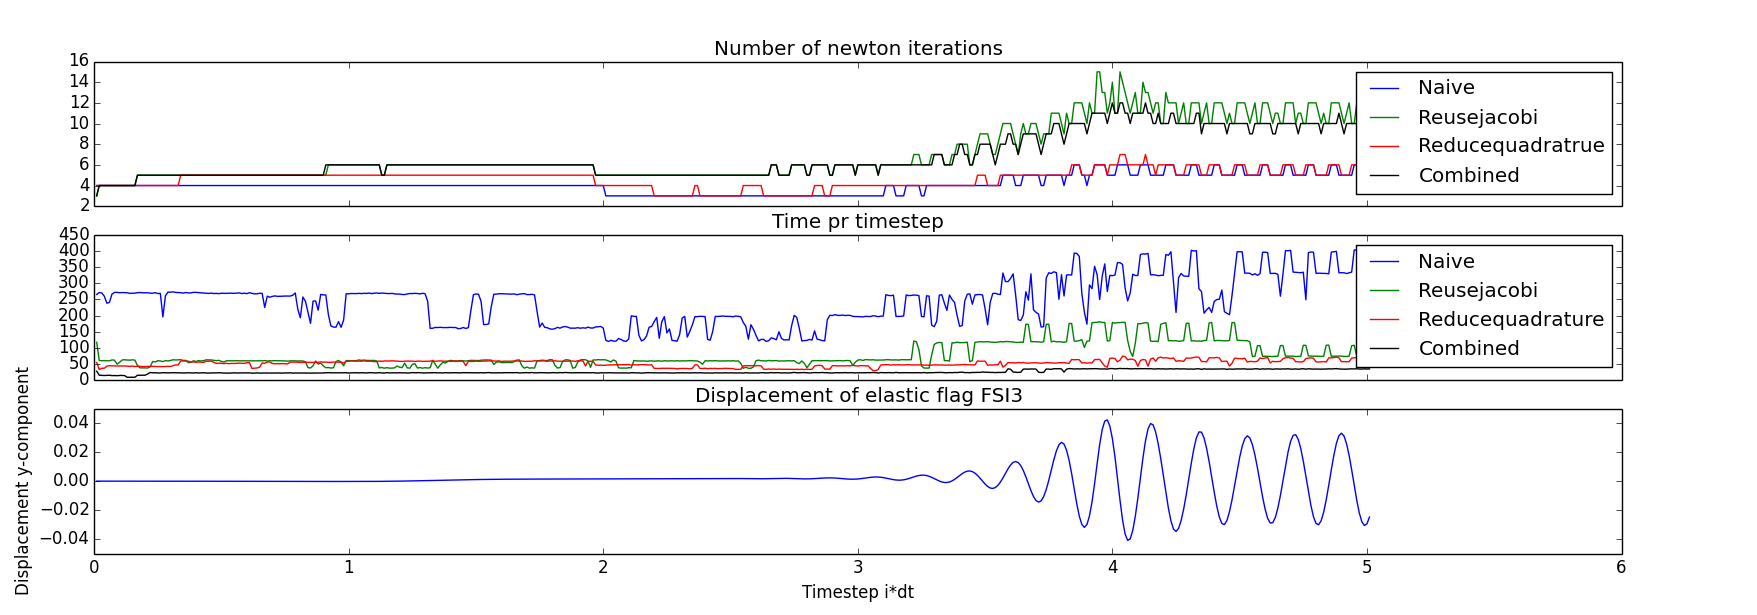
\includegraphics[scale=0.38]{./Fig/bi_compareit.png}
 \begin{tabular}{ |p{2.8cm}|p{2.2cm}|p{2.4cm}|p{2.4cm}|p{2.4cm}|p{2.4cm}| }
 \hline
  \multicolumn{6}{|c|}{Biharmonic Type 1} \\
 \hline
Implementation & Naive & Buffering & Reusejacobi & Reducequad &Combined \\
\hline
 Mean time pr timestep &243.39  & 307.67  & 76.77  & 51.64  & 24.87  \\
\hline
Mean iteration &4.14  & 6.21  & 7.19  & 4.67  & 6.81  \\
\hline
Speedup ration& -  & -0.26  & 0.68  & 0.79  & 0.90  \\
\hline
\end{tabular}
 \caption{Comparison of speed-up techniques for the biharmonic type 1 mesh model.}
  \label{fig:bi_it}
\end{figure}
\subsubsection{Discussion}
Of the speed-up methods considered in this thesis, the combined method proved to fastest for both mesh models. With a computational time difference of nearly $\sim$ 2 hours, the Laplace model is superior to the biharmonic model in terms of efficiency. As long as mesh regularity isn't critical for the simulation, the Laplacian model is the preferable mesh moving model. It is important to note that the introduced speed-up methods may not be applicable to other FSI problems, since inexact Jacobian methods are highly sensitive. 
